%%%%%%%%%%%%%%%%%%%%%%%%%%%%%%%%%%%%%%%%%%%%%%%%%%%%%%%%%%%%%%%%%%%%%
%
% CSCI 1430 Writeup Template
%
% This is a LaTeX document. LaTeX is a markup language for producing
% documents. Your task is to fill out this
% document, then to compile this into a PDF document.
%
% TO COMPILE:
% > pdflatex thisfile.tex
%
% For references to appear correctly instead of as '??', you must run
% pdflatex twice.
%
% If you do not have LaTeX and need a LaTeX distribution:
% - Departmental machines have one installed.
% - Personal laptops (all common OS): www.latex-project.org/get/
%
% If you need help with LaTeX, please come to office hours.
% Or, there is plenty of help online:
% https://en.wikibooks.org/wiki/LaTeX
%
% Good luck!
% James and the 1430 staff
%
%%%%%%%%%%%%%%%%%%%%%%%%%%%%%%%%%%%%%%%%%%%%%%%%%%%%%%%%%%%%%%%%%%%%%
%
% How to include two graphics on the same line:
%
% \includegraphics[\width=0.49\linewidth]{yourgraphic1.png}
% \includegraphics[\width=0.49\linewidth]{yourgraphic2.png}
%
% How to include equations:
%
% \begin{equation}
% y = mx+c
% \end{equation}
%
%%%%%%%%%%%%%%%%%%%%%%%%%%%%%%%%%%%%%%%%%%%%%%%%%%%%%%%%%%%%%%%%%%%%%%%%%%%%%%%%%%%%%%%%%%%%%%%%

\documentclass[11pt]{article}

\usepackage[english]{babel}
\usepackage[utf8]{inputenc}
\usepackage[colorlinks = true,
            linkcolor = blue,
            urlcolor  = blue]{hyperref}
\usepackage[a4paper,margin=1.5in]{geometry}
\usepackage{stackengine,graphicx}
\usepackage{fancyhdr}
\setlength{\headheight}{15pt}
\usepackage{microtype}
\usepackage{times}
\usepackage{booktabs}
\usepackage{amssymb}

% python code format: https://github.com/olivierverdier/python-latex-highlighting
\usepackage{pythonhighlight}

\frenchspacing
\setlength{\parindent}{0cm} % Default is 15pt.
\setlength{\parskip}{0.3cm plus1mm minus1mm}

\pagestyle{fancy}
\fancyhf{}
\lhead{Homework Writeup}
\rhead{CSCI 1430}
\rfoot{\thepage}

\date{}

\title{\vspace{-1cm}Homework Writeup}


\begin{document}
\maketitle
\vspace{-2cm}
\thispagestyle{fancy}

\section*{Instructions}

\begin{itemize}
  \item This write-up is intended to be `light'; its function is to help us grade your work and not to be an exhaustive report.
  \item Be brief and precise.
  \item Please describe any non-standard or interesting decisions you made in writing your algorithm.
  \item Show your results and discuss any interesting findings.
  \item List any extra credit implementation and its results.
  \item Feel free to include code snippets, images, and equations. Below are useful markup templates for these.
  \item \textbf{Please make this document anonymous.}
\end{itemize}

\newpage
% ------------------------------------------------ %

\section*{Declaration of Generative AI Use}

\subsection*{Reminder of Course Policy}

\begin{itemize}
    \item The use of GenAI tools (e.g., ChatGPT, Grammarly, Bard) for completing any part of this course is discouraged.
    \item Using these tools is not needed to be successful in the class and could be detrimental to your learning experience.
    \item If you use them, you must cite the tool you used and explain how you used it.
    \item If you do not cite the tool, it is an academic code violation.
    \item We will be using special tools to detect cases of unattributed GenAI use.
\end{itemize}

\subsection*{Student Declaration}

\subsubsection*{Have you used generative AI tools to complete this assignment:}

%%%%%%%%%%%%%% TODO %%%%%%%%%%%%%%%%%%%%

YES $\square$ NO $\blacksquare$ % change answer to \blacksquare

%%%%%%%%%%%%%%%%%%%%%%%%%%%%%%%%%%%%%%%%

\subsubsection*{If you answered YES above, describe what tools you used and what parts of the assignment you used them for below:}

%%%%%%%%%%%%%% TODO %%%%%%%%%%%%%%%%%%%%

\textit{Example: I used ChatGPT to debug my convolution implementation}

%%%%%%%%%%%%%%%%%%%%%%%%%%%%%%%%%%%%%%%%

% ------------------------------------------------ %
\newpage

\section*{Assignment Overview}

The assignment was to program an image filter that takes in an image and a kernel and produces a modified final image, in our case a hybrid image that merged two images into a final image
that combined the low frequencies of one and the high frequencies of the other.

\section*{Implementation Detail}

I created a convolution function that takes in an image and runs convolution on all of its channels (works the same for RGB and BW). It then stacks the channels back up into the shape
of the original image. It pads the images using zeroes. Numpy.multiply and numpy.sum was used to get the new value for each pixel.

Hybrid image uses this convolution function to create a low pass image and a high pass image and then adds them together. Nothing too interesting happened there.

\section*{Result}

\begin{enumerate}
    \item Behold my beasts...
    \begin{figure}[h]
        \centering
        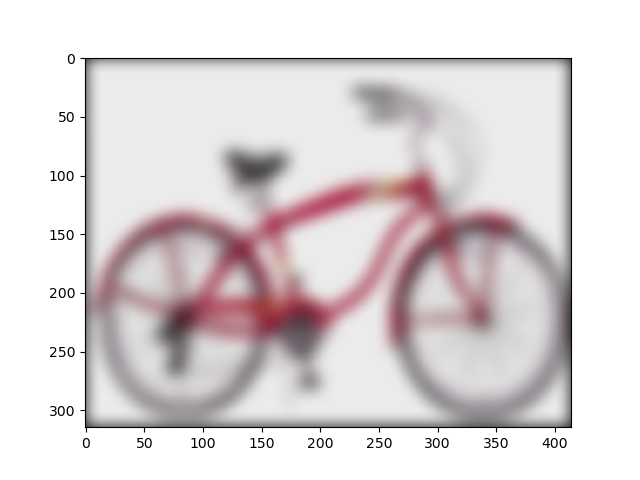
\includegraphics[width=5cm]{lowpassBike.png}
        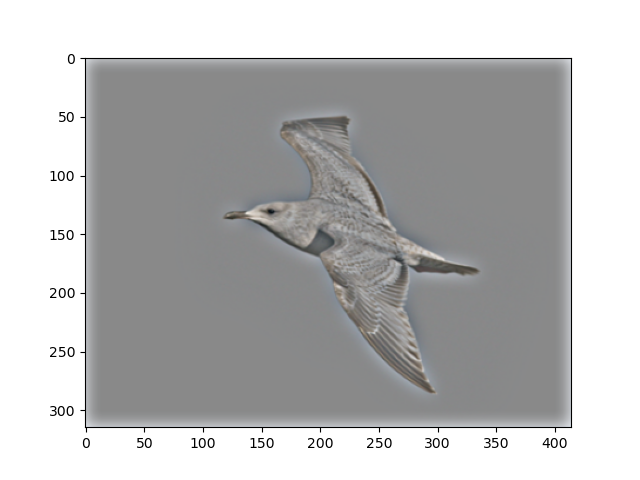
\includegraphics[width=5cm]{highpassBird.png}
        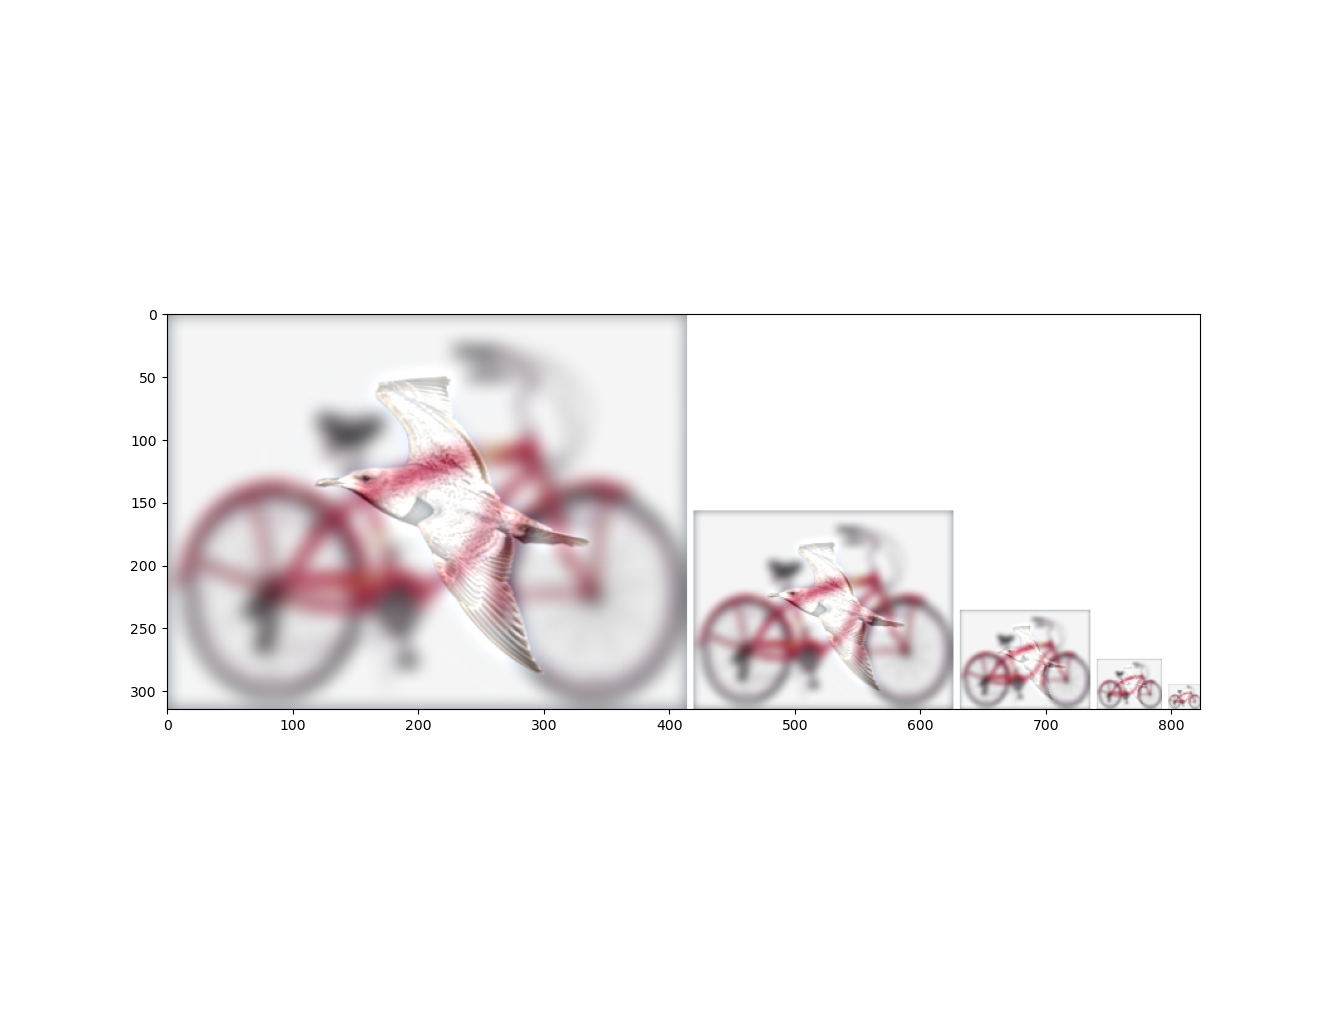
\includegraphics[width=5cm]{birdCycle.png}
        \caption{Combination of a bike and a bird.}
        \label{fig:result1}
    \end{figure}

    \begin{figure}[h]
        \centering
        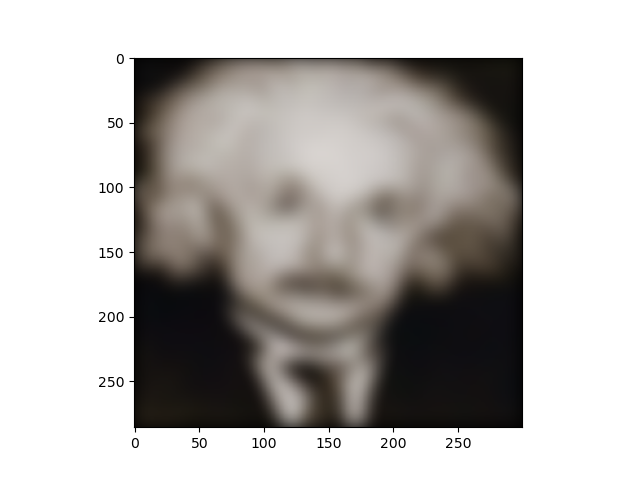
\includegraphics[width=5cm]{lowpassEin.png}
        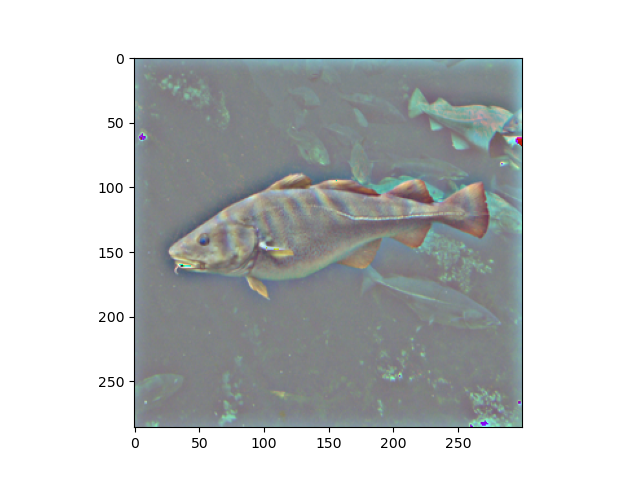
\includegraphics[width=5cm]{highpassFish.png}
        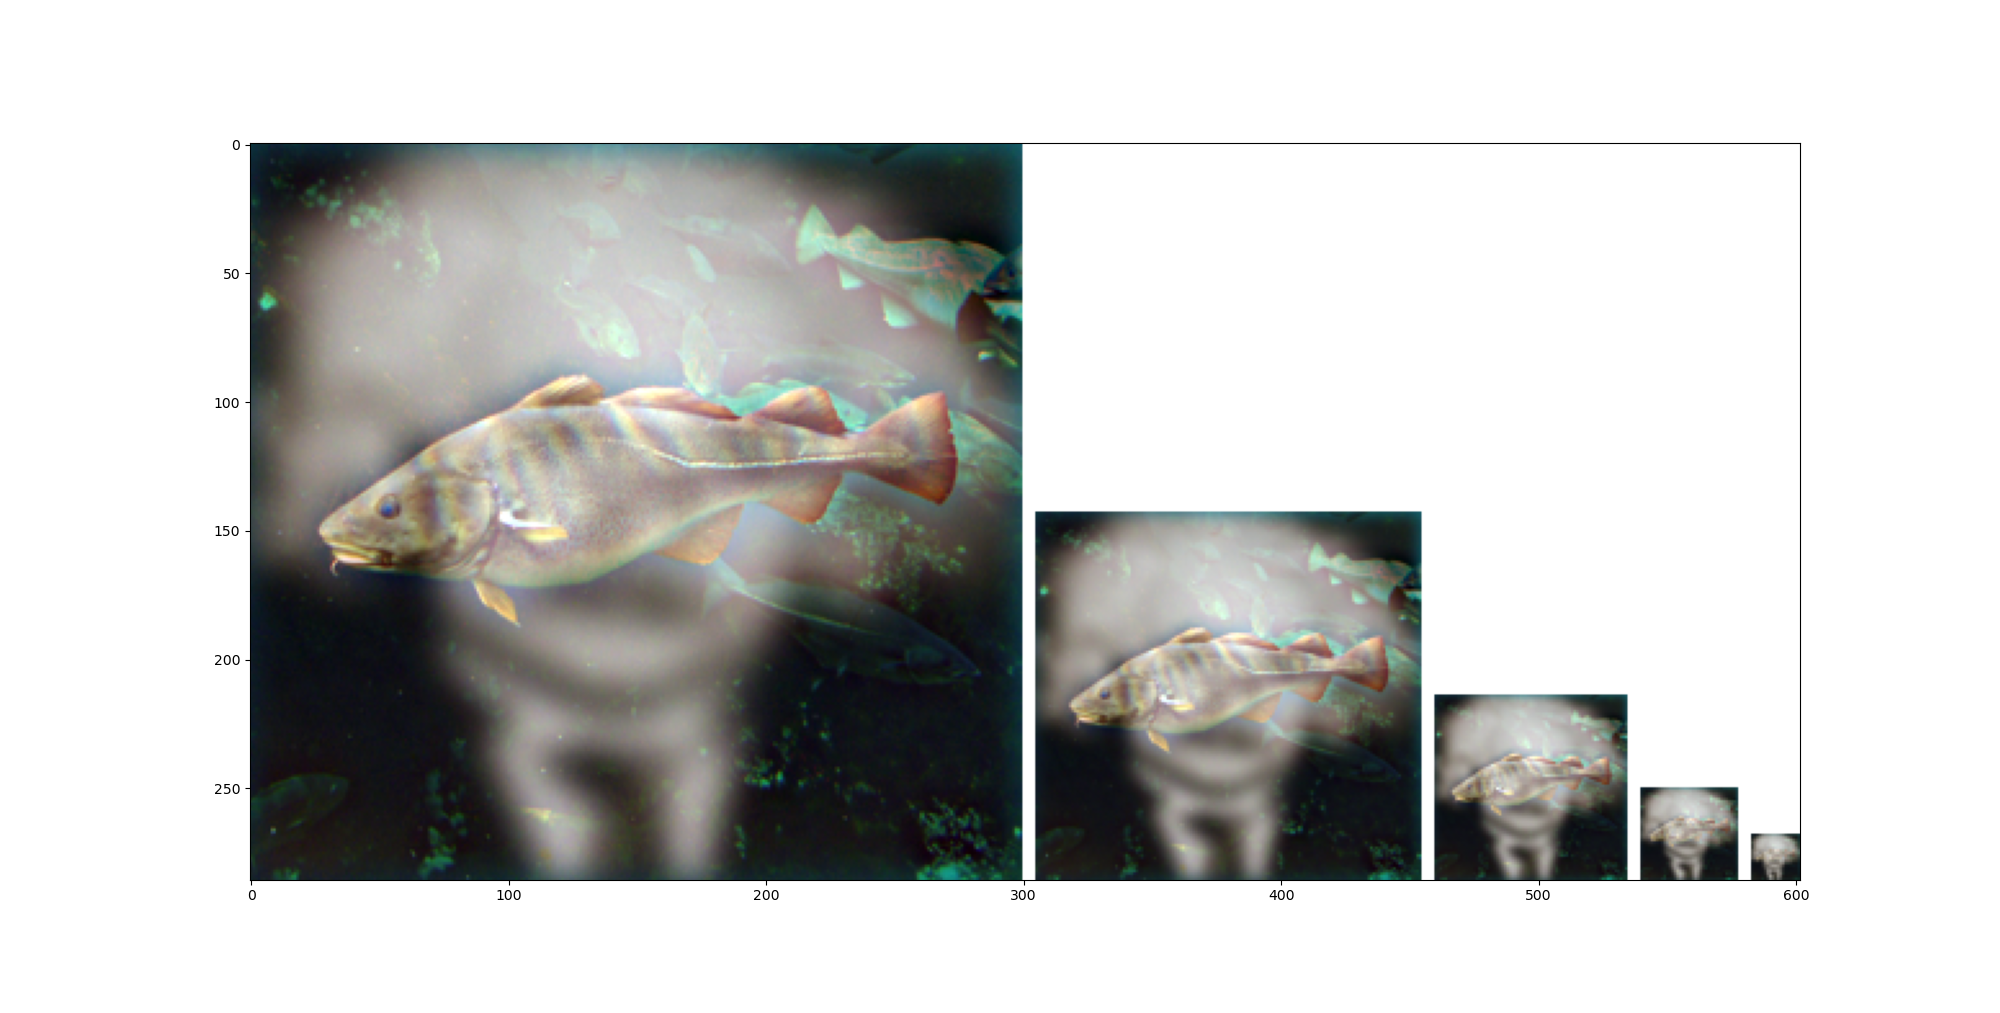
\includegraphics[width=5cm]{fishStein.png}
        \caption{Combination of Einstein and a fish.}
        \label{fig:result2}
    \end{figure}

    \begin{figure}[h]
        \centering
        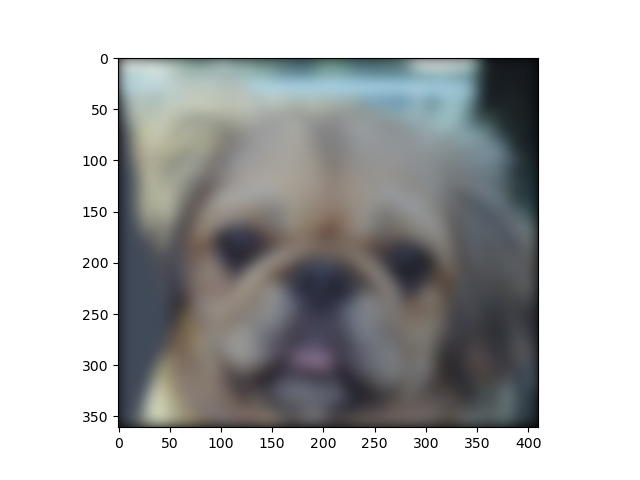
\includegraphics[width=5cm]{lowpassDog.png}
        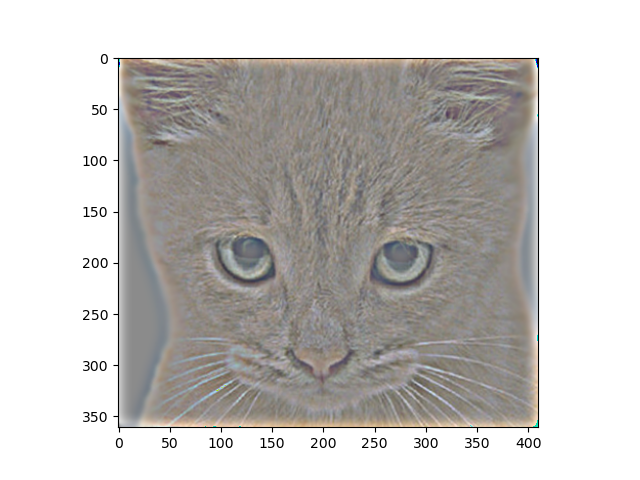
\includegraphics[width=5cm]{highpassCat.png}
        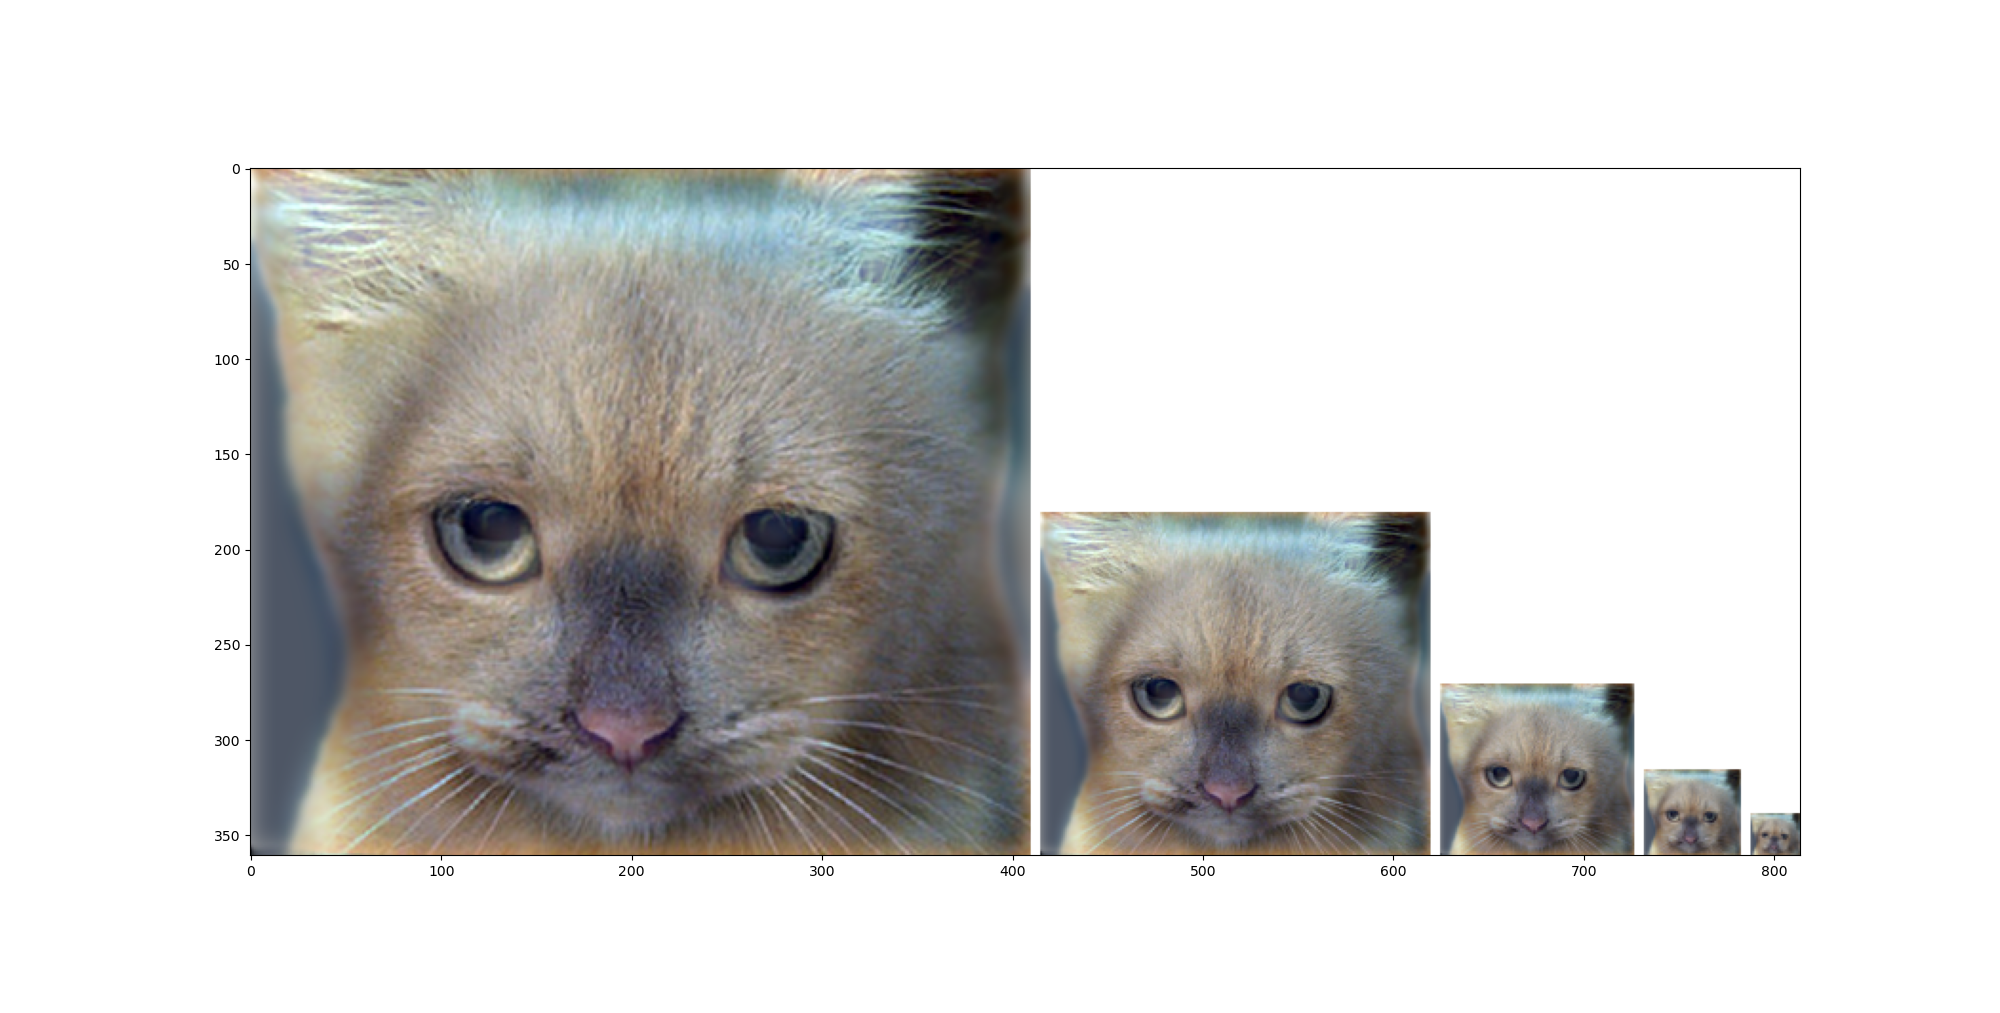
\includegraphics[width=5cm]{catDog.png}
        \caption{Combination of a dog and a cat.}
        \label{fig:result3}
    \end{figure}

\end{enumerate}


\section*{Extra Credit (Optional)}
\begin{enumerate}
   
    \item I formed a hybrid from two images not in the code database: You Know I Had To Do It To Em, and a face from Detective Pikachu.
        
    \begin{figure}[h]
        \centering
        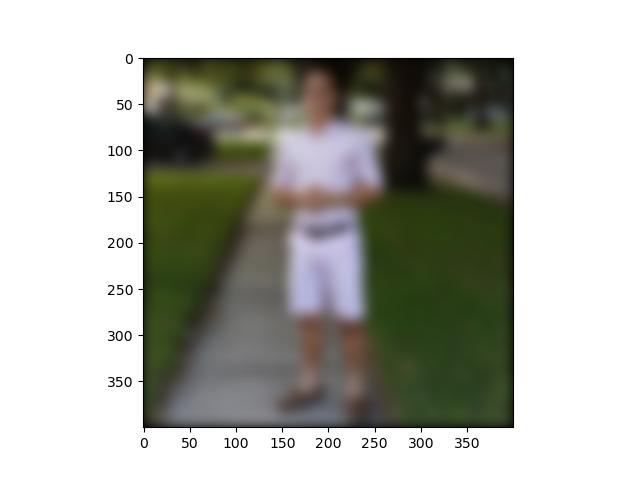
\includegraphics[width=5cm]{lowpassDoit.png}
        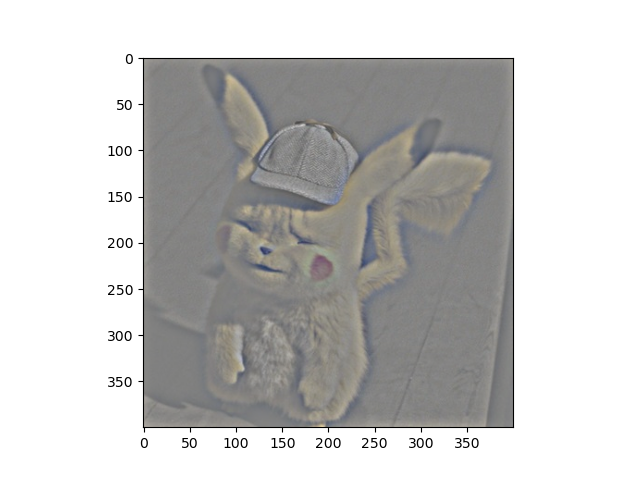
\includegraphics[width=5cm]{highpassPika.png}
        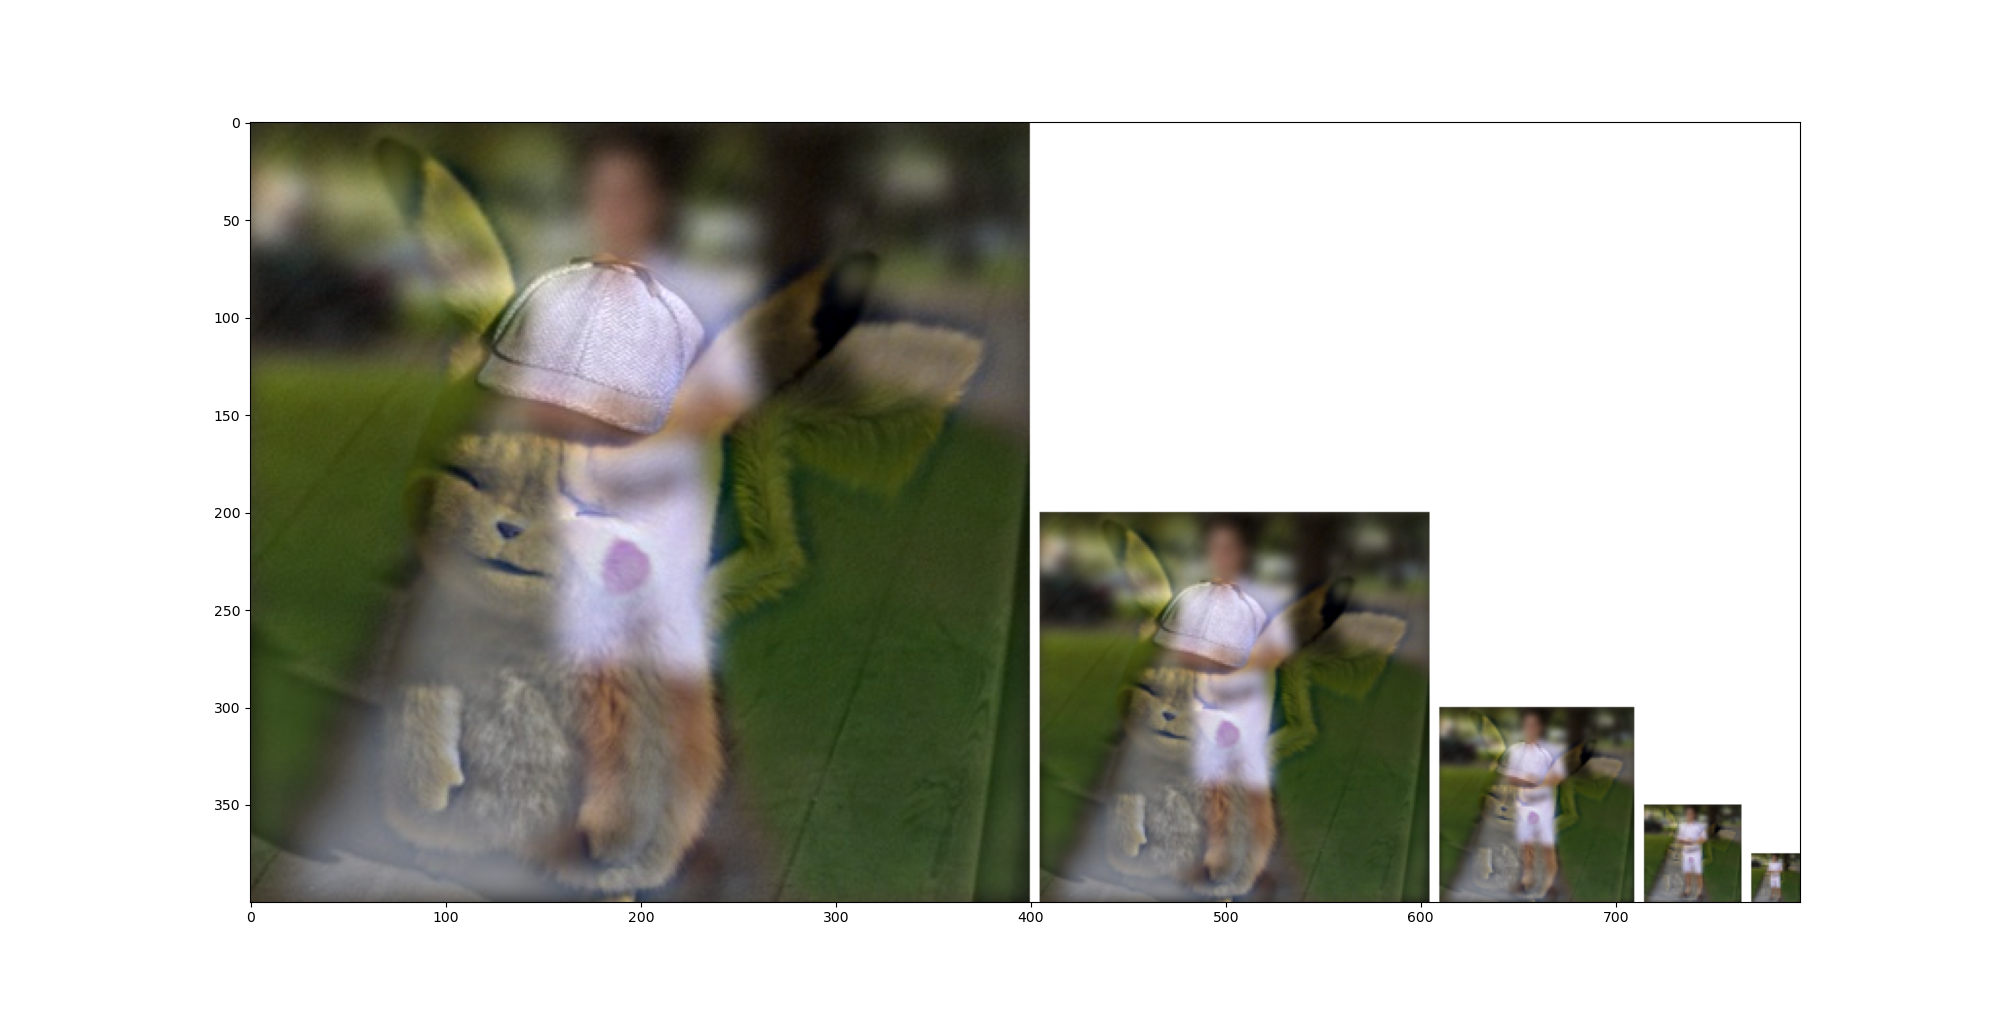
\includegraphics[width=8cm]{splitPika.png}
        \caption{The aforementioned beast.}
        \label{fig:result4}
    \end{figure}

\end{enumerate}

\end{document}
